\documentclass{article}
\usepackage{neurips_style}
\usepackage[utf8]{inputenc}
\usepackage{amsmath,amssymb,amsthm}
\usepackage{booktabs}
\usepackage{graphicx}
\usepackage{xcolor}
\usepackage[colorlinks=true,allcolors=blue]{hyperref}
\usepackage{url}
\usepackage[round,authoryear]{natbib}

\newtheorem{proposition}{Proposition}
\newcommand{\TODO}[1]{\textcolor{red}{\textbf{[TODO: #1]}}}
\newcommand{\MSEo}{\mathrm{MSE}_{\mathrm{ovl}}}
\newcommand{\MSEc}{\mathrm{MSE}_{\mathrm{copy}}}
\newcommand{\MSEf}{\mathrm{MSE}_{\mathrm{fut}}}

\title{How much does a windowed forecast metric flatter you?\\
A closed-form bound, and a corrected EEG benchmark}

\author{%
  \TODO{author block --- anonymised for submission} \\
}

\date{}

\begin{document}
\maketitle

\begin{center}\small\colorbox{yellow!25}{%
\parbox{0.92\textwidth}{\textbf{DRAFT --- not submission-ready.} The argument and
Sections 3--4 are complete and backed by committed artifacts. Sections 5--6 are
scaffolded and marked \TODO{}; see \S8 for exactly what must run first. Do not
circulate as a finished paper.}}\end{center}

\begin{abstract}
A forecasting model is only forecasting if its target is not contained in its
input. We show that a widely used windowed evaluation --- predicting a length-$W$
target window displaced $H<W$ samples from a length-$W$ input window --- scores
$W-H$ positions that are present in the input verbatim, and derive the resulting
inflation of the reported error in closed form. The inflation factor is bounded
above by $W/H$, a quantity computable from the window length and horizon reported
in a methods section, with no access to data, code, or model. We verify the bound
on 286 configurations across 11 signals spanning EEG, ECG, blood pressure,
respiration, and synthetic processes, and observe no violation; agreement with the
exact expression is at machine precision, and departures from the bound are
monotone in a single measurable correction term. The bound holds on white noise,
where nothing is predictable, establishing that the effect is a property of the
scoring rule rather than of the signal. This failure mode is orthogonal to
train/test leakage: it survives subject-wise partitioning, nested
cross-validation, and non-overlapping strides, because it occurs \emph{within} a
single example. We then rescore a sleep-EEG forecasting benchmark under
strictly-future evaluation on 78 subjects, and find that a recurrent model beats a
per-horizon-tuned linear autoregressive baseline out to 160\,ms
($p=2.2\times10^{-6}$ Holm-corrected, 26 of 27 held-out subjects) with the
advantage vanishing by 320\,ms. A control on a synthetic process whose optimal
predictor is provably linear confirms the apparatus does not manufacture wins.
\TODO{one sentence of prevalence result once \S5 runs}
\end{abstract}

\section{Introduction}

Reported gains in machine learning are frequently traceable to evaluation rather
than to modelling. \citet{mcgreivy2024} reviewed machine-learning approaches to
fluid PDEs and found that 79\% (60/76) of papers claiming to outperform a
numerical method compared against a weak baseline. \citet{lin2019} and
\citet{yang2019} made the same argument for neural information retrieval, showing
most reported gains disappeared against strong baselines. In EEG specifically,
\citet{wu2025} reviewed 149 seizure-prediction studies and identified ``few linear
baselines'' as one of four persistent field-wide failures.

We report a distinct and, to our knowledge, undocumented mechanism, in which the
metric itself is at fault rather than the comparator. Consider the common
construction in which a model receives a length-$W$ window and predicts a
length-$W$ window displaced $H$ samples into the future. When $H<W$, the target
window shares $W-H$ samples with the input. A model that learns to shift its input
scores near-zero error on those positions, and the reported mean is dominated by
them.

This is not train/test leakage. Leakage is information crossing the partition
boundary, and the field has a mature literature on preventing it
\citep{bernett2024,apicella2024}, including a large-scale comparison of
cross-validation schemes for EEG over $10^5$ trained models \citep{delpup2025}.
The failure we describe occurs inside a single training example and is invariant
to how examples are assigned to splits. Every remedy in that literature leaves it
intact.

\paragraph{Contributions.}
\begin{enumerate}\itemsep2pt
\item A closed-form expression for the inflation induced by windowed forecast
scoring, and the bound $W/H$, computable from a methods section alone (\S3).
\item Verification on 286 configurations over 11 signals with zero violations,
including on white noise, where the absence of predictable structure isolates the
effect to the scoring rule (\S4).
\item \TODO{prevalence survey of published EEG forecasting protocols (\S5)}
\item A corrected sleep-EEG benchmark with per-subject paired statistics against a
baseline tuned to convergence, locating the horizon at which a nonlinear model
ceases to beat a linear one (\S6).
\end{enumerate}

\section{Related work}

\paragraph{Leakage.} \citet{bernett2024} give seven questions for preventing
leakage in biological machine learning; none concerns overlap between a regression
target and its own input. \citet{delpup2025} compare five cross-validation
settings across more than $10^5$ trained EEG models and establish subject-wise and
nested schemes as necessary. \citet{lee2023} quantify inflation from overlapping
cross-validation under cropping augmentation. \citet{dehghani2019} show that the
apparent benefit of overlapping sliding windows in activity recognition is an
artifact of subject-dependent validation. \citet{wosiak2025} argue that window
shift should be treated as a first-class reported parameter. All concern
information shared \emph{between} examples.

\paragraph{Weak baselines.} \citet{mcgreivy2024}, \citet{lin2019} and
\citet{yang2019} establish the audit-of-a-field genre we follow in \S6.
\citet{beck2025} show that on volatile series no method consistently beats the
naive no-change forecast, motivating our persistence baseline.

\paragraph{EEG forecasting.} \citet{pankka2024} forecast resting-state EEG
150\,ms ahead with a probabilistic WaveNet, outperforming an autoregressive model
on amplitude and phase. \citet{onojima2025} predict the complex analytic signal
from raw multichannel EEG, beating an AR baseline within and across subjects. We
do not claim novelty for deep models outperforming AR at these horizons; our
benchmark contribution is the horizon-resolved crossover against a converged
baseline.

\section{The inflation law}

\subsection{Setup}

Let $s \in \mathbb{R}^{W+H}$ be a signal segment, $W$ the window length and
$1\le H<W$ the horizon. Define
\begin{equation}
X = s[0{:}W], \qquad Y = s[H{:}H{+}W],
\end{equation}
both of length $W$. Since $Y[k]=s[H+k]$ and $X[j]=s[j]$, we have $Y[k]=X[k{+}H]$
whenever $k<W-H$. Partition the target indices into
\begin{equation}
\mathcal{C}=\{0,\dots,W{-}H{-}1\} \;(\text{copyable}), \qquad
\mathcal{F}=\{W{-}H,\dots,W{-}1\} \;(\text{strictly future}),
\end{equation}
with $|\mathcal{C}|=W-H$ and $|\mathcal{F}|=H$. For a single model producing a
single prediction $\hat{Y}$, write $\MSEo$, $\MSEc$ and $\MSEf$ for the mean
squared error over all indices, over $\mathcal{C}$, and over $\mathcal{F}$
respectively. Only the scoring mask differs between the three.

\subsection{The bound}

\begin{proposition}\label{prop:law}
For any predictor and any data distribution, with $\MSEf>0$,
\begin{equation}
\rho \;\equiv\; \frac{\MSEf}{\MSEo}
\;=\; \frac{W/H}{\,1+\frac{W-H}{H}\cdot\frac{\MSEc}{\MSEf}\,}
\;\le\; \frac{W}{H},
\label{eq:law}
\end{equation}
with equality if and only if $\MSEc=0$.
\end{proposition}

\begin{proof}
The mean over $\mathcal{C}\cup\mathcal{F}$ is the weighted mean of the parts:
$\MSEo = \bigl[(W{-}H)\MSEc + H\,\MSEf\bigr]/W$. Dividing $\MSEf$ by this and
factoring $H/W$ gives the stated equality. Since $\MSEc\ge0$ the denominator is at
least $1$, giving the bound; it equals $1$ exactly when $\MSEc=0$.
\end{proof}

Proposition~\ref{prop:law} is an identity, not an approximation: it follows from
the definition of an arithmetic mean and assumes nothing about the model, the
signal, or the estimator. Two consequences are practical. First, $\rho$ is bounded
by $W/H$, which depends only on the evaluation protocol and is therefore
recoverable from a methods section. Second, the bound is one-sided --- a reported
result can never exceed it --- so $W/H$ may be quoted as a worst case without
qualification.

\paragraph{Tightness.} The bound is attained when the model reproduces the
copyable positions exactly. Since those positions are present in the input
verbatim, any model with sufficient capacity to learn an index shift approaches
$\MSEc\to0$, and hence $\rho\to W/H$. Crucially this requires no predictable
structure in the signal.

\section{Verification}

\paragraph{Protocol.} We sweep $W\in\{32,64,128,256\}$ and
$H\in\{1,2,4,8,16,32,64,128\}$ with $H<W$, giving 26 configurations per signal.
Signals: three Sleep-EDF channels (Fpz-Cz, Pz-Oz, EOG), four MIT-BIH
polysomnographic channels (ECG, blood pressure, O2-A1 EEG, nasal respiration), and
four synthetic processes (white noise, AR(1) with $\phi\in\{0.5,0.95\}$, random
walk), for 286 cells. Each cell fits a multi-output ridge, selecting the penalty on
held-out data under the full-window objective --- the criterion the flawed protocol
would itself use --- then scores the resulting predictions under the three masks.
The decomposition in Proposition~\ref{prop:law} is asserted numerically per cell,
so an incorrect mask fails loudly rather than producing a plausible curve.

\begin{figure}[t]
\centering
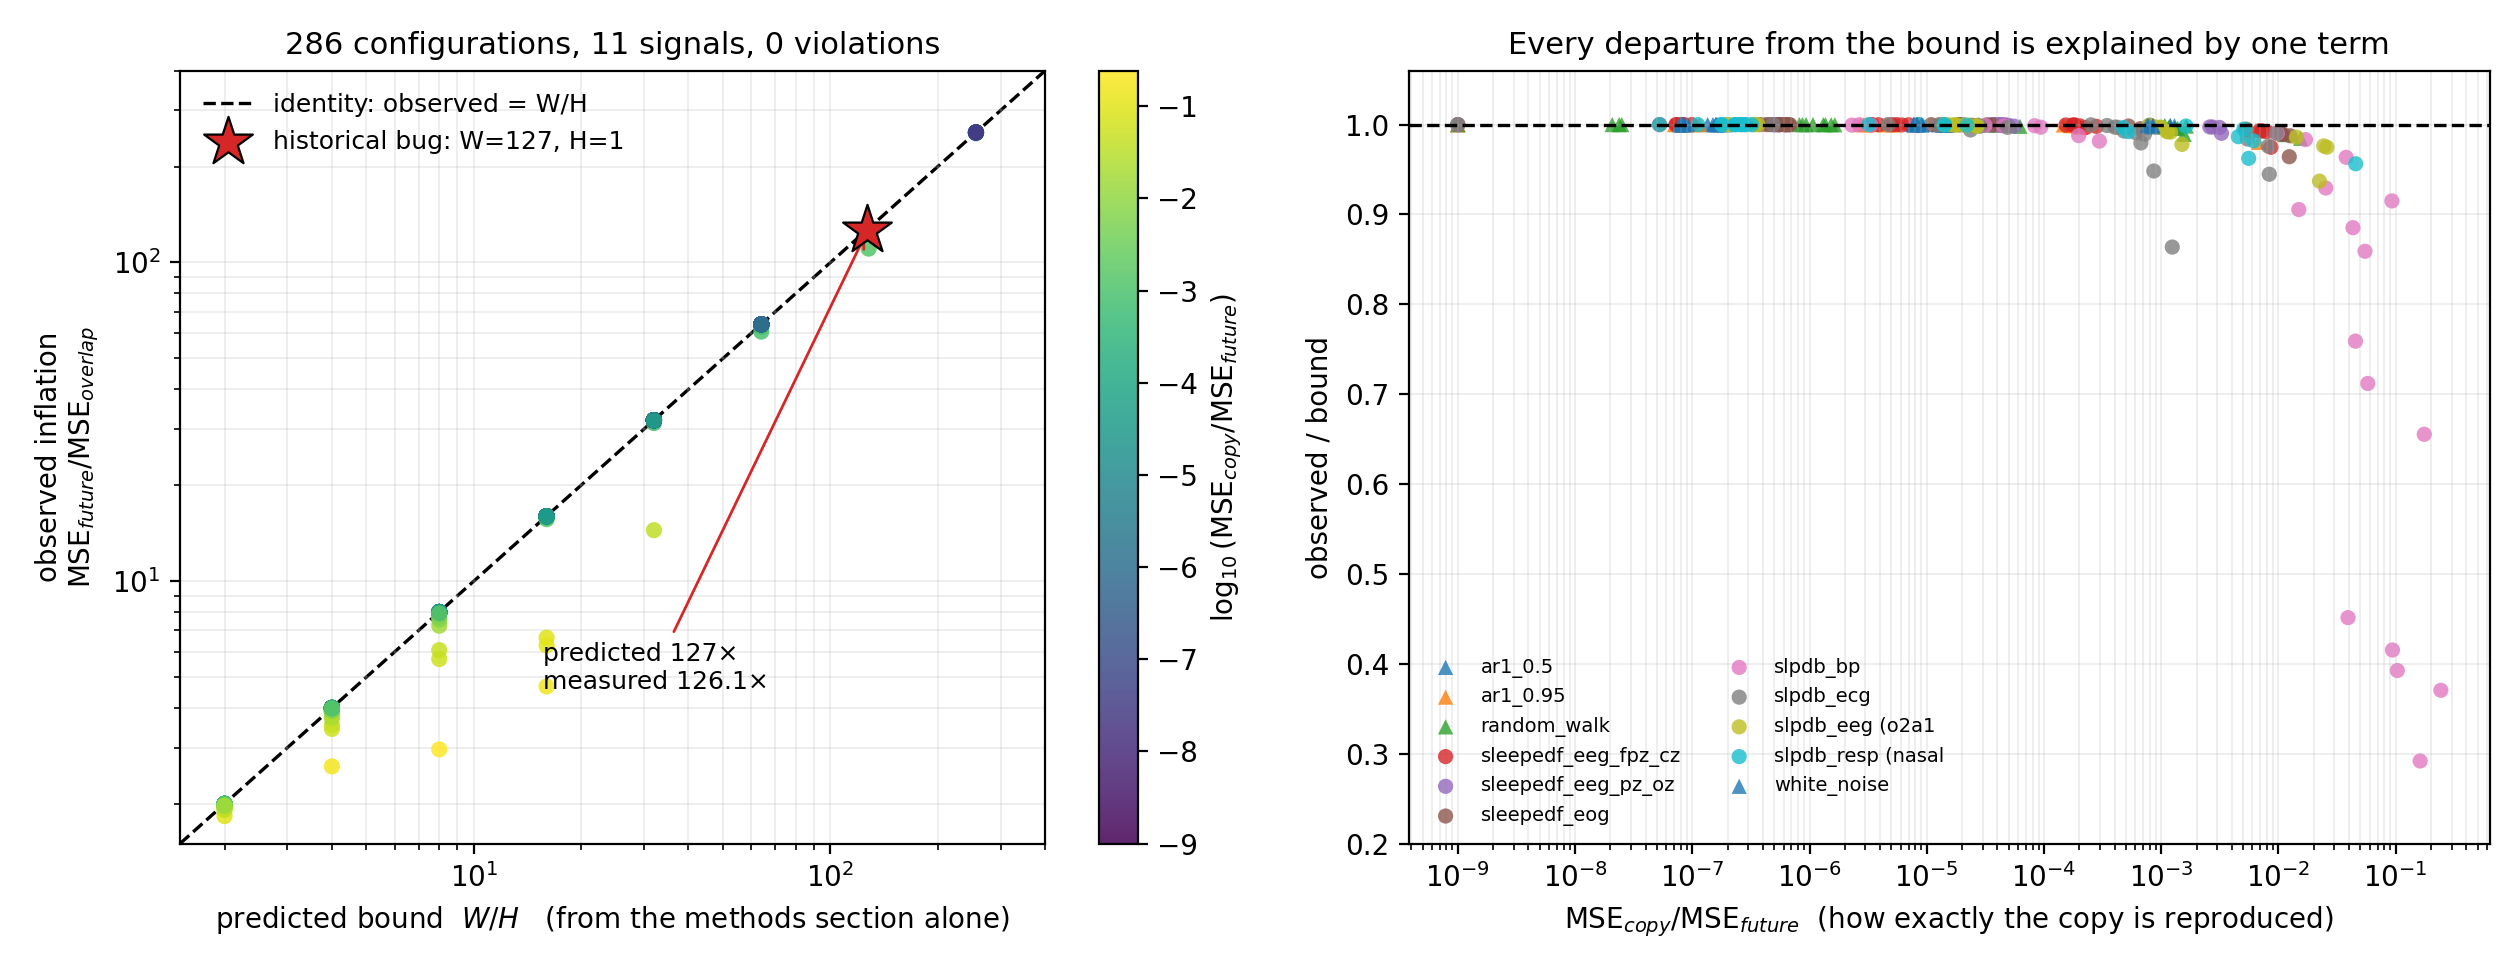
\includegraphics[width=0.95\textwidth]{overlap_law.png}
\caption{\textbf{Left:} predicted bound $W/H$ against observed inflation $\rho$
(log--log) with the identity line. Points lie on the line and never above it; the
region a counterexample would occupy is empty. Colour encodes $\MSEc/\MSEf$. The
star marks a previously published-in-repo result ($W{=}127$, $H{=}1$) for which the
bound predicts $127\times$ and the measured inflation was $126.1\times$.
\textbf{Right:} departure from the bound against $\MSEc/\MSEf$, monotone over five
decades. Triangles synthetic, circles real recordings.}
\label{fig:law}
\end{figure}

\paragraph{Results.} Zero of 286 cells violate the bound. Median $\rho/(W/H)$ is
$1.000$ and the mean $0.981$; the exact expression in \eqref{eq:law} matches the
observed $\rho$ to a maximum relative error of $1.3\times10^{-15}$, as expected for
an identity. Departures are monotone in $\MSEc/\MSEf$: mean $\rho/(W/H)$ is
$1.000$ below $10^{-5}$ (126 cells), $0.986$ over $10^{-3}$--$10^{-2}$ (38 cells),
and $0.428$ above $10^{-1}$ (4 cells). Figure~\ref{fig:law} shows both.

\paragraph{White noise.} On i.i.d.\ Gaussian noise, where no predictor can beat the
mean, median $\rho/(W/H)=1.000$. The copyable positions remain exactly
reproducible because they are present in the input, irrespective of predictability.
This isolates the effect to the scoring rule.

\section{How prevalent is this?}

\TODO{This section is the difference between a tool and a finding about the field,
and it has not been run. Protocol: sample $N\!\approx\!80$ EEG forecasting papers
from 2018--2026 via a systematic search; for each, extract the reported input
window length and prediction horizon; code whether $H\ge W$, $H<W$, or
unrecoverable from the text; report the distribution and the implied $W/H$ for the
$H<W$ subset. Report inter-rater agreement on a subsample. This mirrors
\citet{mcgreivy2024}, and the ``unrecoverable'' rate is itself a reporting-standards
result.}

\section{A corrected benchmark}

\paragraph{Protocol.} Sleep-EDF sleep-cassette, all 78 subjects, subject-disjoint
39/12/27 split with both nights of a subject held together. The task is a
strictly-future single-sample forecast, so input and target share no samples at any
horizon. Baselines: mean-of-window, persistence, and a ridge autoregression whose
penalty is swept per horizon on the validation subjects over a grid extended until
no horizon selects an edge. The recurrent model receives a matched architecture and
step-budget sweep on the same subjects, then three seeds. Error is computed per
test subject, giving paired comparisons; we report Wilcoxon signed-rank with
Holm correction over nine horizons and a 10{,}000-draw bootstrap interval.

\begin{table}[t]
\centering\small
\caption{Mean per-subject MSE on 27 held-out subjects (z-scored units).
$\Delta = \text{ridge} - \text{GRU}$; positive favours the GRU.}
\begin{tabular}{rrrrrrr}
\toprule
$H$ & ms & persistence & ridge-AR & GRU & $\Delta$ & Holm $p$ \\
\midrule
1   & 10   & 0.4322 & 0.2958 & \textbf{0.2754} & $+0.0204$ & $1.0\times10^{-4}$ \\
4   & 40   & 0.5691 & 0.4399 & \textbf{0.3950} & $+0.0450$ & $1.3\times10^{-7}$ \\
16  & 160  & 1.3814 & 0.8298 & \textbf{0.7268} & $+0.1031$ & $2.2\times10^{-6}$ \\
32  & 320  & 1.7600 & \textbf{0.8700} & 0.8756 & $-0.0056$ & n.s. \\
64  & 640  & 2.0433 & \textbf{0.8771} & 0.9004 & $-0.0234$ & $1.2\times10^{-4}$ \\
256 & 2560 & 1.8746 & \textbf{0.9942} & 1.0099 & $-0.0157$ & $1.3\times10^{-7}$ \\
\bottomrule
\end{tabular}
\label{tab:bench}
\end{table}

\paragraph{Result.} The recurrent model is superior out to 160\,ms, where it is
12.4\% below the tuned linear baseline on 26 of 27 subjects and 47.4\% below
persistence. The advantage is absent from 320\,ms onward. The crossover, not the
margin, is the reportable quantity: it locates where nonlinearity ceases to pay.

\paragraph{Baseline tuning changes the conclusion.} With the ridge penalty fixed at
an arbitrary constant, the 160\,ms comparison favoured the recurrent model by 16\%;
with a search grid truncated below the optimum, the same comparison reversed. Only
after extending the grid until the selected penalty was interior did the result
stabilise. We report this because it is a second inflation mechanism, independent
of \S3, and because both of our own early configurations would have produced a
publishable but incorrect claim.

\paragraph{Controls.} We report eight, of which two are load-bearing. On a
stationary AR(2) process, where the minimum-MSE predictor is provably linear, the
same recurrent model with the same tuning budget \emph{loses} to ridge
($p=0.014$), establishing that the apparatus does not manufacture wins for the
model under test. A linear model trained with the recurrent model's exact optimiser
and step budget is worse than the closed-form ridge at every horizon, excluding the
explanation that the margin reflects optimisation rather than architecture.
Label-permutation and noise-input controls both collapse to the variance floor.

\paragraph{A claim that did not survive.} We initially reported that the tuned
ridge beats the recurrent model at 640\,ms ($p=4.1\times10^{-5}$). Under fully
non-overlapping windows this becomes a tie ($p=0.58$). We therefore claim only that
the recurrent advantage ends by 320\,ms, not that the linear model wins beyond it.

\section{Limitations}

The bound governs the metric and is silent on model quality: a strong and a useless
model inflate identically. It assumes the shifted-window construction of \S3;
other overlapping constructions require their own copyable-position count, after
which the same identity applies. The benchmark in \S6 uses a single EEG channel and
a single corpus, and the horizon at which the advantage ends (160\,ms) is roughly
$400\times$ shorter than the timescale relevant to clinical state prediction. We
make no clinical claim. \TODO{remove this sentence once \S5 lands: the prevalence
of the protocol in published work is not yet established, so we characterise the
bound as a tool rather than a finding about the field.}

\section{What must run before submission}

\TODO{Delete this section before submitting; it is a working checklist.}
\begin{enumerate}\itemsep2pt
\item \textbf{Prevalence survey (\S5).} Blocking. Without it the paper is a
methods note. $\sim$80 papers, two coders, reported agreement.
\item \textbf{Second and third corpora for \S6.} \texttt{chbmit},
\texttt{siena-scalp-eeg} and \texttt{eegmmidb} are referenced in the repository
but not downloaded; a single-corpus benchmark is not defensible at this venue.
\item \textbf{A third and fourth model class.} Currently ridge versus GRU. A
temporal convolutional network and a transformer are the minimum for a claim about
nonlinearity in general.
\item \textbf{Multichannel.} \citet{onojima2025} beat AR using multichannel input;
our single-channel setup is the most likely reason the crossover occurs so early,
and testing it is the highest-value scientific experiment remaining.
\item \textbf{Anonymisation and the official style file.} This draft uses a local
approximation of the NeurIPS layout.
\end{enumerate}


\begin{thebibliography}{99}\small
\bibitem[Apicella et al.(2024)]{apicella2024} Apicella, A., et al. (2024). Don't push the button! Exploring data leakage risks in machine learning and transfer learning. \emph{Artificial Intelligence Review}.
\bibitem[Beck et al.(2025)]{beck2025} Beck, N., et al. (2025). Mind the naive forecast! A rigorous evaluation of forecasting models for time series with low predictability. \emph{Applied Intelligence}.
\bibitem[Bernett et al.(2024)]{bernett2024} Bernett, J., et al. (2024). Guiding questions to avoid data leakage in biological machine learning applications. \emph{Nature Methods}.
\bibitem[Dehghani et al.(2019)]{dehghani2019} Dehghani, A., et al. (2019). A quantitative comparison of overlapping and non-overlapping sliding windows for human activity recognition using inertial sensors. \emph{Sensors}.
\bibitem[Del Pup et al.(2025)]{delpup2025} Del Pup, F., et al. (2025). The role of data partitioning on the performance of EEG-based deep learning models in supervised cross-subject analysis. \emph{Computers in Biology and Medicine}.
\bibitem[Lee et al.(2023)]{lee2023} Lee, H.-T., et al. (2023). Risk of data leakage in estimating the diagnostic performance of a deep-learning-based computer-aided system for psychiatric disorders. \emph{Scientific Reports}.
\bibitem[Lin(2019)]{lin2019} Lin, J. (2019). The neural hype and comparisons against weak baselines. \emph{ACM SIGIR Forum}.
\bibitem[McGreivy \& Hakim(2024)]{mcgreivy2024} McGreivy, N., \& Hakim, A. (2024). Weak baselines and reporting biases lead to overoptimism in machine learning for fluid-related partial differential equations. \emph{Nature Machine Intelligence}.
\bibitem[Onojima et al.(2025)]{onojima2025} Onojima, T., et al. (2025). Direct prediction of the complex-valued analytic signal of EEG from raw multichannel data. \emph{bioRxiv}.
\bibitem[Pankka et al.(2024)]{pankka2024} Pankka, H., et al. (2024). Enhanced EEG forecasting: a probabilistic deep learning approach. \emph{bioRxiv}.
\bibitem[Puffay et al.(2023)]{puffay2023} Puffay, C., et al. (2023). Relating EEG to continuous speech using deep neural networks: a review. \emph{Journal of Neural Engineering}.
\bibitem[Wosiak et al.(2025)]{wosiak2025} Wosiak, A., et al. (2025). Impact of temporal window shift on EEG-based machine learning models for cognitive fatigue detection. \emph{Algorithms}.
\bibitem[Wu et al.(2025)]{wu2025} Wu, Y., et al. (2025). A review of machine learning and deep learning trends in EEG-based epileptic seizure prediction. \emph{IEEE Access}.
\bibitem[Yang et al.(2019)]{yang2019} Yang, W., et al. (2019). Critically examining the ``neural hype'': weak baselines and the additivity of effectiveness gains from neural ranking models. \emph{SIGIR}.
\end{thebibliography}

\end{document}
